\documentclass[11pt, oneside]{article}   	% use "amsart" instead of "article" for AMSLaTeX format
\usepackage[margin = 1in]{geometry}                		% See geometry.pdf to learn the layout options. There are lots.
\geometry{letterpaper}                   		% ... or a4paper or a5paper or ... 
%\geometry{landscape}                		% Activate for rotated page geometry
%\usepackage[parfill]{parskip}    		% Activate to begin paragraphs with an empty line rather than an indent
\usepackage{graphicx}				% Use pdf, png, jpg, or eps§ with pdflatex; use eps in DVI mode
								% TeX will automatically convert eps --> pdf in pdflatex		
\usepackage{amssymb}
\usepackage{amsmath}
\usepackage[shortlabels]{enumitem}
\usepackage{float}
\usepackage{subcaption}
\usepackage{tikz-cd}
\usepackage{tikz}

\usepackage{amsthm}
\theoremstyle{definition}
\newtheorem{definition}{Definition}[section]
\newtheorem{theorem}{Theorem}[section]
\newtheorem{corollary}{Corollary}[theorem]
\newtheorem{lemma}[theorem]{Lemma}
\newtheorem{prop}{Prop}[section]

\newcommand{\N}{\mathbb{N}}
\newcommand{\R}{\mathbb{R}}
\newcommand{\Z}{\mathbb{Z}}
\newcommand{\Q}{\mathbb{Q}}

%SetFonts

%SetFonts


\title{Representation Theory}
\author{Patrick Oare}
\date{}							% Activate to display a given date or no date

\begin{document}
\maketitle

These notes will cover the basics of representation theory and its applications to physics. Most of the 
theory that we discuss will have a large range of applications, and you will almost certainly see it in 
a course on quantum field theory. This subject is integral to all of physics because representation 
theory provides a mathematical framework to study symmetries, both discrete and continuous. 
Whenever a physicist says the words ``group theory" he or she really means ``representation theory", and 
it really is impossible to study subjects like quantum field theory without at least a working knowledge 
of representation theory. 

Although I'm writing these notes as a background for physics, I tend to write my notes more like a 
mathematician. As such, there will be some sections that read like definition, definition, theorem, 
corollary. I've found that bundling things up into theorems make them easier to remember and reference 
in the long run, and this is ultimately meant to be a reference for myself to use when doing physics. 
Generally, I will only include proofs of theorems if I find them to be informative or fun to do, so if a 
proof is there, it is generally pretty easy or will introduce methods that will be used later. We will 
assume background knowledge in algebra (specifically group theory and linear algebra) and some 
knowledge of topology, specifically smooth manifolds. 

Now for some common notation. For a field $\mathbb K$, we let  $M_{n\times m}(\mathbb K)$ 
denote the set of all $m\times n$ matrices with values in $\mathbb K$ (usually here $\mathbb K$ will 
be either $\mathbb R$ or $\mathbb C$). Group representations will typically be denoted by $\Pi$ or 
by $D$ depending on whether the group is a Lie group or finite group, and Lie algebra representations 
will typically be denoted $\pi$. For algebraic objects $M$ and $N$ (by this I mean objects in a category), 
the set of morphisms between them will be denoted $Hom(M, N)$.

Let $V$ be a $n$-dimensional $\mathbb K$-vector space. We denote its dual by $V^*$, and recall for 
finite dimensional vector spaces there is an isomorphism $V\rightarrow V^*$. An \textbf{endomorphism} 
of $V$ is an homomorphism $\phi : V\rightarrow V$. If $\phi$ is invertible (an isomorphism $V\rightarrow 
V$) then we will call $\phi$ an \textbf{automorphism}. We will denote its automorphism group of $V$ by $Aut(V)$ 
and its endomorphism ring by $End(V)$. The group $Aut(V)$ is naturally isomorphic to the group 
$GL(V) := GL(\mathbb K^n)$ of $n\times n$ invertible matrices with values in $\mathbb K$ (as once 
a basis is chosen for $V$, invertible linear maps $V\rightarrow V$ are in bijection with invertible matrices), 
and the group $End(V)$ is naturally isomorphic to $gl(V) := gl(\mathbb K^n)$, the set of all $n\times n$ 
matrices with values in $\mathbb K$. 

Most of these notes will go over general theory with occasional examples in each section to provide insight into 
when these theorems and definitions will be relevant in physics. We will primarily be discussing Lie groups, but 
after discussing Lie groups there will be some sections on the representation theory of finite groups and character 
theory. We will also explicitly delve into some important examples for physics, including the representation theory 
of $SU(N)$, the Poincar\'e group, and the hypercubic group.

\newpage
\section{Lie Groups, Algebras and Representations}

Lie groups are used to describe sets of continuous symmetries. Although we will attempt to 
make definitions as general as possible, we will often restrict ourselves to the case of specific 
examples which are of interest for physics, namely the Lie groups $SU(N)$, $SO(N)$, and 
occasionally symplectic groups, which is where classical mechanics lives. We define Lie groups 
and algebras, and then will discuss the 
interplay between the two.

\begin{definition}[Lie group]
	A \textbf{Lie group} $(G, \cdot)$ is a group which is also a differentiable manifold, in which the 
	group operation respects the structure of the manifold. Namely, we require that the maps 
	$\cdot : G^2\rightarrow G$ and $\cdot^{-1} : G\rightarrow G$ be smooth.
\end{definition}

\begin{definition}[Lie algebra]
	A \textbf{Lie algebra} $\mathfrak g$ over a field $k$ is a $k$-valued vector space equipped with 
	a map $[\cdot, \cdot] : \mathfrak g\times\mathfrak g\rightarrow\mathfrak g$, called a \textbf{Lie 
	bracket}, such that the following hold:
	\begin{enumerate}
		\item $[\cdot, \cdot]$ is bilinear.
		\item $[\cdot, \cdot]$ is antisymmetric. 
		\item $[\cdot, \cdot]$ satisfies the \textbf{Jacobi identity}, i.e. for $A, B, C\in\mathfrak g$:
		\begin{equation}
			[A, [B, C]] + [B, [C, A]] + [C, [A, B]] = 0
		\end{equation}
	\end{enumerate}
\end{definition}

We will generally be considering matrix Lie groups and algebras, in which case the Lie bracket is 
simply the commutator, $[A, B] = AB - BA$. In the case of matrix groups, our Lie algebras will 
also be matrix-valued, so $\mathfrak g$ is a matrix-valued vector space. We call it an algebra 
because the map $[\cdot, \cdot]$ gives the vector space an algebra-like structure\footnote{An 
algebra is simply a vector space with a ring structure, i.e. with a multiplication $\cdot : \mathfrak 
g\times \mathfrak g \rightarrow\mathfrak g$. However, the axioms that ring multiplication must satisfy 
are different than those that $[\cdot, \cdot]$ must satisfy.}.

The essential idea behind Lie groups is this: Lie groups act on a vector space $V$ as the symmetry 
operation (for example, the group $SO(3)$ of orthogonal real valued $3\times 3$ matrices with 
determinant 1 act as rotations in $V = \mathbb R^3$). Lie algebras generate the Lie group via the 
exponential map in the following way: suppose $U\in G$ 
is an arbitrary element (assume $G$ is path-connected, or at least that $U$ is in the path-component 
of $1\in G$). Then, there exists $X\in\mathfrak g$ such that:
\begin{equation}
	U = \exp(iX)
\end{equation}
The proof of this existence is one of the fundamental theorems of Lie theory, and is why we care 
about Lie algebras. In essence, the Lie algebra parameterizes the Lie group. Let $n = dim(\mathfrak 
g)$. If we pick a basis 
$\{T^a\}_{a = 1}^n$ for $\mathfrak g$, the elements of this basis are called \textbf{generators} of the 
Lie group $G$ because an arbitrary element of $G$ can be represented as:
\begin{equation}
	\exp(i X^a T^a)
\end{equation}
because $T^a$ spans $\mathfrak g$. This means the coordinates $X^a$ parameterize the Lie 
group $G$ (really they parameterize the path-component of 1), and so we can specify an 
element of $G$ by specifying a set of $n$ coordinates. 

Every Lie algebra is defined by its Lie bracket. Since $[\cdot, \cdot]$ maps $\mathfrak g^2$ into 
$\mathfrak g$, we must be able to expand:
\begin{equation}
	[T^a, T^b] = if^{abc}T^c
\end{equation}
where $f^{abc}$ is an antisymmetric tensor of numbers known as the \textbf{structure constants} 
of the Lie algebra. Specifying the structure constants of an algebra exactly define the algebra and 
its Lie bracket. 

The associated Lie algebra with a Lie group can be defined by taking its tangent space at the 
identity, and in this way we have an correspondence from Lie groups to Lie algebras, and back. 
Geometrically, I like to view a (connected) Lie group as a ``smoothly deformed version" of a flat Lie algebra. 
The exponential map does the deformation, and to me this emphasizes the fact that a Lie group is 
first and foremost a manifold. 

A common operation on Lie algebras we will use is the adjoint operation, of which there are two; the 
first is an action from the element of the Lie algebra, and the second is from the action of the Lie group. 
For $X\in\mathfrak g$, we define the \textbf{adjoint map} $ad_X : \mathfrak g\rightarrow\mathfrak g$ by:
\begin{equation}
	ad_X(Y) := [X, Y]
\end{equation}
For $A\in G$, there is a different type of adjoint map that we can consider. It is still an endomorphism of 
$\mathfrak g$, just defined slightly differently. Here we also require $G$ to be a matrix Lie group so that 
we can multiply elements of the algebra with elements of $G$. The map is denoted $Ad_A : \mathfrak g
\rightarrow\mathfrak g$:
\begin{equation}
	Ad_A(Y) := AYA^{-1}
\end{equation}
and we see that it is just the group adjoint. These two maps are connected via the exponential map:
\begin{equation}
	e^{ad_X} = Ad_{e^{X}}
\end{equation}
which is an expression of the familiar formula for Lie algebras:
\begin{equation}
	e^{X} Y e^{-X} = Y + [X, Y] + \frac{1}{2}[X, [X, Y]] + ...
\end{equation}

To act Lie groups on spaces, we must discuss representations. Note that the endomorphism ring 
$End(V)$ of a vector space is also a Lie algebra, by allowing the Lie bracket to equal the commutator 
of operators $A, B\in End(V)$. 
\begin{definition}[Representation]
	A \textbf{representation} of a Lie algebra $\mathfrak g$ on a vector space $V$ is a Lie 
	algebra homomorphism\footnote{Meaning it preserves $+$ and $[\cdot, \cdot$]}  
	$\mathfrak g\rightarrow End(V)$. A representation of a Lie group $G$ is a Lie group 
	homomorphism $G\rightarrow Aut(V)$, where $Aut(V)$ denotes the space of vector space 
	automorphisms on $V$. If a representation is injective then we call it \textbf{faithful}, in which 
	case different group elements map to different matrices in $Aut(V)$. 
\end{definition}

\begin{definition}[Dimension]
	The \textbf{dimension} of a representation $\pi : G\rightarrow Aut(V)$ is the dimension of $V$. 
	If $\pi : G\rightarrow GL(n, \mathbb F)$ is a representation of a Lie group with $n\times n$ matrices, 
	then $n$ is the dimension of $\pi$. 
\end{definition}

\begin{definition}[Equivalent representations]
	Two representations $\Pi : G\rightarrow Aut(V)$ and $\Psi : G\rightarrow Aut(V)$ are said to be 
	\textbf{equivalent} if there is $S\in Aut(V)$ such that:
	\begin{equation}
		\Pi(g) = S\Pi(g) S^{-1}~
		\label{eq:equivalent}
	\end{equation}
\end{definition}

Equivalent representations are essentially the same representation, since a conjugation like in 
Equation~\ref{eq:equivalent} is the same as changing the basis that the two representations are 
expanded in. 

 A representation can likewise be defined as an action of $G$ or $\mathfrak g$ on $V$, as given a 
representation $\pi : \mathfrak g\rightarrow V$, we have a $\mathfrak g$-action on $V$ defined 
by $X\cdot v := \pi(X)(v)$. The easiest way to define a representation is to give an explicit 
embedding of the generators of $\mathfrak g$ into $End(V)$ as matrices, as every endomorphism 
can be realized as a matrix. Once the generators are embedded into matrices, then the rest of 
the representation can be embedded by linearity. Here are a few more definitions to keep in mind. 

Representations are more than just a Lie group and a vector space: they also implicitly contain the 
map from $G\rightarrow Aut(V)$. Because of this, we have been labelling a representation $\Pi : G\rightarrow 
Aut(V)$ as $\Pi$ WLOG. However, we also may label the representation by the triple $(\Pi, G, V)$ 
(and similarly for an algebra representation we may label it as $(\pi, \mathfrak g, V)$. Since each 
$G$-representation induces a canonical $\mathfrak g$-representation (and vice versa), it is often 
useful to abuse notation and to let $V$ denote the $G$-representation and the $\mathfrak g$-representation, 
since $V$ is the common element of the triple denoting $\Pi$ and $\pi$. This is often used in physics, where 
for example we may refer to the octet of $SU(3)$ as $\textbf{8}$ to denote the representation $\pi : \mathfrak{su}(3)
\rightarrow\mathbb R^8$ which has action $\pi(T^a)^{bc} = - if^{abc}$ (the adjoint representation).  

We now consider what a morphism between representations looks like. This is called an intertwining map, and 
is essentially a vector space map which respects the action induced by the representation. 

\begin{definition}[Intertwining map]
	Let $\Pi : G\rightarrow Aut(V)$ and $\Sigma : G\rightarrow Aut(W)$ be two representations of a Lie group $G$, 
	and let $\phi : V\rightarrow W$ be a linear map. We call $\phi$ an \textbf{intertwining map} if for each $g\in G$ 
	and $v\in V$ we have:
	\begin{equation}
		\phi(\Pi(g) v) = \Sigma(g) (\phi v)
	\end{equation}
	In other words, the canonical diagram commutes for each element $g\in G$:
	\[\begin{tikzcd}
		V\arrow[r, "\Pi(g)"]\arrow[d, "\phi"] & V\arrow[d, "\phi"] \\
		W\arrow[r, "\Sigma(g)"] & W
	\end{tikzcd}\]
	An intertwining map which is invertible is a \textbf{representation isomorphism}. 
\end{definition}

An intertwining map is simply a morphism in the category of representations: it preserves both the linear 
structure of the spaces it acts on and the action of the representation. A more obvious way to view such a map 
is as follows: denote by $\cdot$ the action of $G$ on $V$ or $W$, i.e. $g\cdot v := \Pi(g)v$. Then the definition of 
$\phi$ being an intertwining map can equivalently be written as:
\begin{equation}
	\phi(g\cdot v) = g\cdot \phi(v)
\end{equation}
which makes it completely obvious that such an intertwining map is a morphism in the category of linear 
$G$-representations. 

\subsection{Algebras vs. Groups}
Let $G$ be a Lie group with associated Lie algebra $\mathfrak g$. We will now discuss to what extent a representation 
of $G$ induces a representation of $\mathfrak g$, and vice versa. 
\begin{definition}
	Let $\mathfrak g$ and $\mathfrak h$ be two Lie algebras. A \textbf{Lie algebra homomorphism} between $\mathfrak g$ 
	and $\mathfrak h$ is a linear map $\phi : \mathfrak g\rightarrow\mathfrak h$ which respects the Lie bracket, i.e. 
	$\phi([X, Y]) = [\phi(X), \phi(Y)]$ for each $X, Y\in\mathfrak g$. 
\end{definition}
On the other hand, a Lie group homomorphism is simply a group homomorphism which is smooth with respect to 
the manifold structure of the group. However, there is a subtle disparity between Lie groups and Lie algebras when 
it comes to maps between them. Lie algebras are simpler objects than Lie groups because they have a fundamentally 
linear structure. This means that if two Lie groups are the same, then their Lie algebras will be the same; unfortunately, 
the converse only holds in certain cases where the Lie group has a simple structure. Recall that we can move between 
$\mathfrak g$ and $G$ by exponentiation, $X\mapsto \exp(iX)$, and consider the following theorem.
\begin{theorem}
	Let $G$ and $H$ be Lie groups with algebras $\mathfrak g$ and $\mathfrak h$, and let $\Phi : G\rightarrow H$ be a 
	Lie group homomorphism. Then, there is an unique homomorphism of Lie algebras $\phi : 
	\mathfrak g\rightarrow\mathfrak h$ such that:
	\begin{equation}
		\Phi(e^{iX}) = e^{i\phi(X)}
	\end{equation}
	for each $X\in\mathfrak g$. Furthermore, $\phi$ is given by:
	\begin{equation}
		\phi(X) := \frac{d}{dt}\bigg|_{t = 0}\Phi(e^{itX})
	\end{equation}
\end{theorem}
In this theorem lies the disparity; a Lie group homomorphism $\Phi$ induces a Lie algebra homomorphism $\phi$, 
but we have said nothing about the converse. Indeed, the converse is not always true. This associated map also 
acts functorially, in that if $\Phi : H\rightarrow K$ and $\Psi : G\rightarrow H$ are homomorphisms of Lie groups and 
$\Lambda = \Phi\circ\Psi$, then (denoting the map between algebras as lowercase):
\begin{equation}
	\lambda = \phi\circ\psi
\end{equation}
This immediately says that \textbf{if two Lie groups are isomorphic, then so are their Lie algebras}. In particular, 
consider the effect this has on representations of a group.
\begin{corollary}
	Let $\Pi : G\rightarrow Aut(V)$ be a representation of a Lie group $G$. Then there is an associated 
	representation of Lie algebras $\pi : \mathfrak g\rightarrow End(V)$. In other words, every representation 
	of a Lie group induces a representation of its Lie algebra.
\end{corollary}

The converse of this is \textbf{only true when $G$ is simply connected}, i.e. $\pi_1(G) = 0$, and can be proved with 
the Baker-Campbell-Hausdorff formula. 
\begin{theorem}
	Let $G$ and $H$ be Lie groups with Lie algebras $\mathfrak g$ and $\mathfrak h$. Let $\phi : \mathfrak g
	\rightarrow\mathfrak h$ be a homomorphism of Lie algebras. If $G$ is simply connected, then there exists 
	a unique Lie group homomorphism $\Phi : G\rightarrow H$ such that $\Phi(e^{iX}) = e^{i\phi(X)}$. 
\end{theorem}
\begin{corollary}
	Suppose $G$ and $H$ are simply connected Lie groups with Lie algebras $\mathfrak g$ and $\mathfrak h$. If 
	$\mathfrak g$ is isomorphic to $\mathfrak h$, then $G$ is isomorphic to $H$. 
\end{corollary}
\begin{corollary}
	Let $G$ be a Lie group with Lie algebra $\mathfrak g$, and let $\pi : \mathfrak g\rightarrow End(V)$ be a representation 
	of $\mathfrak g$. Suppose that $G$ is simply connected. Then there is a corresponding representation $\Pi : 
	G\rightarrow Aut(V)$ such that $\Pi(e^{iX}) = e^{i\pi(X)}$ for $X\in\mathfrak g$. 
\end{corollary}

As an example of all this, consider the Lie groups $SU(2)$ and $SO(3)$\footnote{$SU(2)$ is the ``universal cover" of $SO(3)$, 
which means that $SU(2)$ is simply connected and has the same Lie algebra as $SO(3)$. I hope to include covering spaces in 
these notes at some point if I have time, because I believe that much of the correspondence between these two spaces 
generalizes to an arbitrary Lie group and its universal cover.}. These have the same Lie algebras, 
but since $SU(2)\cong S^3$, it is simply connected, while $SO(3)$ has $\pi_1(SO(3))\cong\mathbb Z / 2\mathbb Z$. 
Let $\phi : \mathfrak{su}(2)\rightarrow\mathfrak{so}(3)$ be the corresponding Lie algebra isomorphism. 
In a later section we will show that every representation of $\mathfrak{su}(2)$ is of the form $\pi_m : \mathfrak{su}(2)
\rightarrow End(V_m)$ with $dim(V_m) = m + 1$. Then, we of course can form a representation of $\mathfrak{so}(3)$ 
by lifting $\pi_m$ with the isomorphism, $\sigma_m := \pi_m\circ\phi^{-1}$, and these are precisely the isomorphisms 
of $\mathfrak{so}(3)$, since $\mathfrak{so}(2)$ and $\mathfrak{su}(3)$ are the same Lie algebra. Here's the catch: 
if $m$ is even, then there is a representation $\Sigma_m$ of $SO(3)$ such that $\Sigma_m(e^{iX}) = e^{i\sigma_m(X)}$ 
for each $X\in\mathfrak{so}(3)$. However, \textbf{if $m$ is odd, then there is no representation of $SO(3)$ such that 
$\sigma_m$ is the induced Lie algebra representation}. 

You should know this fact inherently from physics: it is the statement that rotating systems with half integral spin behaves 
differently than 3D rotations, i.e. a full $2\pi$ rotation of a spin state is not the identity. The representations of $SU(2)$ are 
exactly the different angular momentum systems; a system with angular momentum $j$ has Hilbert space $V_m$ with 
$m = 2j$, as the dimension of the Hilbert space is $2j + 1 = m + 1$. The angular momentum operators on this Hilbert space 
are $\frac{1}{2}\pi_m(\sigma_i)$, where $\sigma_i$ are the Pauli matrices which generate $\mathfrak{su}(2)$. So, a system 
with integer angular momentum $j$ ($m$ even) has is described representation of $\mathfrak{su}(2)\cong\mathfrak{so}(3)$ 
which is induced by a representation of the 3D rotation group $SO(3)$, and thus these rotations must behave like 3D rotations. 
In the half integer case, there is no corresponding representation $\Sigma_m$ of $SO(3)$, and thus quantum mechanical 
rotations do not need to behave like rotations in $SO(3)$. 

\newpage
\section{Irreducible Representations}

Irreducible representations (irreps) are the simplest representations that one can create-- they are 
akin to simple groups in standard group theory, or prime ideals in ring theory. They will give us a way 
to decompose complicated Lie groups into sums of irreps, which will allow us to study these groups based 
off of studying these simpler substructures. Any representation we are interested in will be able to be 
decomposed into irreps, which makes it quite important to study these irreps in the context of physics. 

\begin{definition}[Irreducible representation]
If $\Pi : G\rightarrow Aut(V)$ is a representation of $G$, we say that a subspace $W\subset V$ is 
an \textbf{invariant subspace} if $\pi(g)(W)\subseteq W$ for each $g\in G$, i.e. that the group 
\textit{always} goes into itself under symmetry transformations. We say that $W$ is \textbf{nontrivial} 
if $W$ is a nonempty proper subspace. If the representation $\pi$ has no nontrivial invariant subspaces, 
then we call $\pi$ an \textbf{irreducible representation}. 
\end{definition}

\begin{definition}[Irreducible subspace]
	Let $\Pi : G\rightarrow Aut(V)$ be a representation of $G$. If $W\subseteq V$ is invariant and if 
	it contains no proper invariant subspaces, then we call $W$ an \textbf{irreducible subspace} of 
	$\Pi$. 
\end{definition}

Note that saying $V$ is an irreducible subspace of itself is the same as saying that the representation $V$ 
is irreducible. Because we are studying Lie theory in the context of physics, we are interested in representations of 
symmetry groups. In particular, these groups are unitary, and so are the representations of these groups.
\begin{definition}[Unitary]
	Let $\Pi : G\rightarrow Aut(V)$ be a representation. Then $\Pi$ is an \textbf{unitary representation} if $\Pi(g)$ 
	is a unitary operator on $V$ for each $g\in G$. Note that this implies $\Pi(g^{-1}) = \Pi(g)^\dagger$. 
\end{definition}

Luckily for us, unitary representations are quite simple and can always be decomposed into the direct sum of irreps. 
We will make this precise with a few definitions.

\begin{definition}[Completely reducible]
	A finite dimensional representation of a Lie group or algebra is \textbf{completely reducible} if it is isomorphic 
	to a direct sum of a finite number of irreps. 
\end{definition}

\begin{prop}
	Let $\Pi : G\rightarrow Aut(V)$ be a completely reducible representation. Then:
	\begin{enumerate}
		\item For each invariant subspace $U\leq V$, $V$ splits as a direct product $V = U\oplus W$ with 
		$W$ also invariant. 
		\item Every invariant subspace of $V$ is completely reducible.
	\end{enumerate}
\end{prop}

The last part of this proposition will allow us to prove that unitary representations are completely reducible, hence 
when studying representations in physics we can build up our representations from irreps without loss of generality.

\begin{theorem}
	Any finite dimensional unitary representation of a Lie group or algebra is completely reducible.
\end{theorem}

\begin{proof}
	Let $\Pi : G\rightarrow Aut(V)$ be unitary. If $\Pi$ is an irrep, then we are done. So, suppose it is not, and pick 
	a nontrivial invariant subspace $W\leq V$. Then $V$ splits as $V = W\oplus W^\perp$. We show that $W^\perp$ 
	is invariant as well. Let $v\in W^\perp$. Then for each $g\in G$ and $w\in W$, we have:
	\begin{equation}
		\langle \Pi(g)v|w\rangle = \langle v | \Pi(g^{-1}) |w\rangle = 0
	\end{equation}
	because $\Pi(g^{-1})|w\rangle\in W$ as $W$ is invariant. So, $\Pi(g)v\in W^\perp$ for each $g\in G$. We 
	can inductively repeat this process on both $W$ and $W^\perp$ a finite number of times until this terminates 
	with each summand being an irrep, and the process must terminate because $V$ is finite dimensional. 
\end{proof}

In addition, finite representations of compact Lie groups are also completely reducible. We will not prove this, but it 
is certainly a nice fact to know.

\begin{theorem}
	If $G$ is compact, then every finite dimensional representation of $G$ is completely reducible.
\end{theorem}

An important theorem about irreps is called \textbf{Schur's lemma}. We will simply state the theorem.
\begin{lemma}[Schur]
	\begin{enumerate}
		\item Let $V$ and $W$ be irreducible real or complex representations of a group or Lie algebra and 
		let $\phi : V\rightarrow W$ be an intertwining map (representation homomorphism). Then $\phi$ 
		is either identically 0 or an isomorphism of representations.
		\item Let $V$ be a complex irrep of a group or Lie algebra and let $\phi : V\rightarrow V$ be an 
		intertwining map. Then $\phi = \lambda I$ for some $\lambda\in\mathbb C$. 
		\item Let $V$ and $W$ be complex irreps of a group or Lie algebra and $\phi_1, \phi_2 : V\rightarrow 
		W$ be nonzero intertwining maps. Then $\phi_1 = \lambda\phi_2$ for some $\lambda\in\mathbb C$. 
	\end{enumerate}
\end{lemma}
Schur's lemma essentially states that any two irreps which are homomorphic are also isomorphic, and so irreps 
are the simplest building blocks of representations. There is also a few nice corollaries which deal with commuting 
objects in the representation.
\begin{corollary}
	Let $(\Pi_1, V), (\Pi_2, V)$ be two inequivalent irreps of $G$. If $\Pi_1(g) A = A\Pi_2(g)$ for each $g\in G$, then 
	$A = 0$. 
\end{corollary}
\begin{corollary}
	Let $(\Pi, V)$ be an irrep of $G$. If $\Pi(g)A = A\Pi(g)$ for each $g\in G$ and $A\in Aut(V)$, then $A = \lambda I$. 
\end{corollary}
\begin{corollary}
	Let $\mathfrak g$ be a Lie algebra and $(\pi, V)$ is an irrep of $\mathfrak g$. If $X$ is in the center of 
	$\mathfrak g$ (so $[X, Y] = 0$ for each $Y\in\mathfrak g$), then $\pi(X) = \lambda I$. 
\end{corollary}
These theorems are all very similar, and the main point is that \textbf{any element in an irrep of $G$ which commutes 
with all other elements of $G$ is proportional to the identity}. This can be a surprisingly powerful fact, and it often 
is applicable in places you might not expect it to be. It also proves the following fact, because if a group is 
commutative then each element must be mapped to a multiple of $I$. 
\begin{corollary}
	An irrep of a commutative group is one dimensional.
\end{corollary}

Finally, we must discuss some notation. We will often denote a representation by its dimension 
by simply writing a number for the representation. For example, the adjoint of $SU(3)$ is 8-dimensional, the fundamental 
and anti-fundamental representations are 3-dimensional, and the singlet (trivial) representation is 1-dimensional. We denote the 
adjoint by $\bf{8}$, the fundamental by $\bf 3$, the anti-fundamental by $\bf{bar 3}$, and the singlet by $\bf 1$. One will often 
see equations written out in physics books that look like:
\begin{equation}
	\bf 3\otimes \bar{3} = 8\oplus 1
\end{equation}
All this means is that if we tensor together the fundamental with the anti-fundamental, it splits as a direct sum of the adjoint 
plus the singlet. We will discuss some of the common irreps of Lie groups in the following subsections.

\subsection{The Adjoint Representation}

The adjoint representation is perhaps the most canonical of representations because every Lie 
algebra admits an adjoint representation on itself. For $X\in\mathfrak g$, recall we defined the adjoint 
map $ad_X : \mathfrak g\rightarrow\mathfrak g$ by:
\begin{equation}
	ad_X(Y) := [X, Y]
\end{equation}
It is easy to show that the map $\mathfrak g\rightarrow End(\mathfrak g)$, $X\mapsto ad_X$ is a 
Lie algebra homomorphism. Thus this must define a representation, called the \textbf{adjoint 
representation} of $\mathfrak g$, in which the elements of $\mathfrak g$ can act on the algebra 
that they span. Suppose that our Lie algebra is $d$ dimensional, so it has $d$ generators $T^a$. 
We can explicitly embed the $T^a$ into the adjoint representation by matrices $T_A^a$. To 
compute these matrices, suppose that we have an element $X = X^a T^a\in\mathfrak g$. Since the 
matrices $T_A^a$ act on the column vector $X^a$, they must be $d\times d$ dimensional. Additionally, 
when $T_A^a$ is multiplied against the vector $X^a$, it must give the components of 
$ad_{T^a}(X)$ (because $T^a_A$ represents the operator $ad_{T^a}$), so:
\begin{equation}
	(ad_{T^a}(X))^b = (T_A^a)^{bc} X^c\iff ([T^a, X^c T^c])^b = iX^c f^{acb} = (T_A^a)^{bc} X^c
\end{equation}
And thus we see that the components of the generators in the adjoint representation must be given by:
\begin{equation}
	(T_A^a)^{bc} = -if^{abc}
\end{equation}

Consider what the transformation law looks like in the adjoint representation. Of course, this is 
a matrix multiplication of $X^a$ by the group element. Let $V = \exp(i\alpha^a T_A^a)$ be an element of 
$G$ in the adjoint representation. Then:
\begin{equation}
	X^a\mapsto (X^a)' = V^{ab}X^b
\end{equation}
by definition. Infinitesimally, this is:
\begin{equation}
	X^a\mapsto (1 + i\alpha^c T_A^c)^{ab} X^b = X^a + i\alpha^c (-if^{cab})X^b = X^a - 
	f^{abc}\alpha^b X^c
\end{equation}

Now for the interesting question: what does the transformation law for the element $X = X^a T^a$ 
look like? We claim that the matrix $X$ actually transforms under conjugation by $V$:
\begin{equation}
	X\mapsto X' = VXV^\dagger
\end{equation}
We can check this by expanding out this transformation law for an infinitesimal $\alpha$:
$$
	X^a T^a\mapsto (1 + i\alpha^a T^a) (X^b T^b) (1 - i\alpha^c T^c) = X + i\alpha^a X^b [T^a, T^b]
	= X - \alpha^a X^bf^{abc}T^c 
$$
$$
	= (X^a - f^{abc}\alpha^b X^c)T^a
$$
which is exactly the transformation law we were looking for. Thus, we can view transformation in the 
adjoint representation in two different ways. First, as how the vector of component fields transforms:
\begin{equation}
	X^a\mapsto V^{ab} X^b
\end{equation}
And secondly, how the entire matrix $X$ transforms:
\begin{equation}
	X\mapsto VXV^\dagger
\end{equation}

\newpage
\section{Constructions}

\subsection{Complexification}

It is often useful to study a real Lie algebra by complexifying it and studying the algebra as a complex 
vector space instead of a real vector space. 
\begin{definition}[Complex Lie group]
	A Lie group $G$ is \textbf{complex} if its Lie algebra $\mathfrak g$ is a vector space over $\mathbb C$, 
	i.e. if $iX\in\mathfrak g$ for each $X\in\mathfrak g$. 
\end{definition}

We will next define how to complexify a real vector space and treat it as a $\mathbb C$-vector space. This 
will extend naturally to any Lie algebra (as a Lie algebra has a vector space structure in addition to its Lie 
bracket) in a functorial manner. 
\begin{definition}[Complexification]
	Let $V$ be a vector space over $\mathbb R$. Then the \textbf{complexification} of $V$, denoted $V_\mathbb{C}$, is the 
	set of formal linear combinations:
	\begin{equation}
		V_\mathbb{C} = \{v_1 + iv_2 : v_1, v_2\in V\}
	\end{equation}
	We endow $V_\mathbb{C}$ with a vector space structure by defining for $v_1 + iv_2\in V_\mathbb{C}$:
	\begin{equation}
		i(v_1 + iv_2) := -v_2 + iv_1
	\end{equation}
	This extends by linearity to all of $V_\mathbb{C}$, making it into a vector space over $\mathbb C$. 
\end{definition}

The complexification of a vector space is in itself also a real vector space of dimension $2dim(V)$, since as a set it is 
isomorphic to the direct sum $V\oplus V$. For a Lie algebra, we can use this construction to complexify the structure of the 
algebra as a vector space, and also extend the bracket to this new complex space. The complexification is also the ``best" way 
we can embed a real Lie algebra into a complex Lie algebra, in the sense that it is a universal attractor in the category of maps 
$\mathfrak g\rightarrow h$, where $h$ is a complex Lie algebra. 

\begin{theorem}
	Let $\mathfrak g$ be a finite dimensional real Lie algebra. Let $\mathfrak g_\mathbb{C}$ be its complexification as a 
	vector space. Then the bracket $[\cdot, \cdot]$ extends uniquely to $\mathfrak g_\mathbb{C}$ by:
	\begin{equation}
		[X_1 + iX_2, Y_1 + iY_2] := ([X_1, Y_1] - [X_2, Y_2]) + i([X_2, Y_1] + [X_1, Y_2])
	\end{equation}
	making $\mathfrak g_\mathbb{C}$ into a Lie algebra. 
\end{theorem}

\begin{prop}
	Let $\mathfrak g\subset M_n(\mathbb C)$ be a real Lie algebra, and suppose that $iX\not\in\mathfrak g$ for $X\in
	\mathfrak g$. Then $\mathfrak g_\mathbb{C}$ is isomorphic to the set of matrices in $M_n(\mathbb C)$ of the form 
	$X + iY$ with $X, Y\in\mathfrak g$. 
\end{prop}

\begin{theorem}
	Let $\mathfrak g$ be a real Lie algebra with complexification $\mathfrak g_\mathbb{C}$, and let $\iota : \mathfrak 
	g\rightarrow\mathfrak g_\mathbb{C}$ be the canonical inclusion. Then $\mathfrak g$ is universal in the sense that if 
	$\mathfrak h$ is any complex Lie algebra and $f : \mathfrak g\rightarrow\mathfrak h$ is a Lie algebra homomorphism, 
	then we can factor $f$ through $\mathfrak g_\mathbb{C}$:
	\[\begin{tikzcd}
		\mathfrak g\arrow[r, "\iota"]\arrow[dr, swap, "f"] & \mathfrak g_\mathbb{C}\arrow[d, "\overline{f}"] \\
		& \mathfrak h \\
	\end{tikzcd}\]
\end{theorem}
Some common complexifications which are useful are:
\begin{itemize}
	\item $\mathfrak u(N)_\mathbb{C}\cong gl(N; \mathbb C)$
	\item $\mathfrak su(N)_\mathbb{C}\cong \mathfrak{sl}(N; \mathbb C)$
\end{itemize}

Complexification leaves irreps invariant, so studying the irreps of a complexified Lie algebra is equivalent to studying the 
irreps of the original algebra. This will be very useful as it will allow us to study the irreps of $\mathfrak{su}(N)$ through the 
irreps of $\mathfrak{sl}(n; \mathbb C)$. 

\begin{theorem}
	Let $\mathfrak g$ be a real Lie algebra with complexification $\mathfrak g_\mathbb{C}$. Then every finite dimensional 
	complex representation $\pi$ of $\mathfrak g$ has a unique extension to a complex representation of 
	$\mathfrak g_{\mathbb C}$ by linearity, also denoted $\pi$. Furthermore, $\pi$ is irreducible as a representation of 
	$\mathfrak g_{\mathbb C}$ iff it is irreducible as a representation of $\mathfrak g$. 
\end{theorem}

\subsection{Sums}

Recall the direct sum $V_1\oplus V_2$ of two vector spaces $V_1$ and $V_2$ is simply a fancy way of writing 
the Cartesian product $V_1\times V_2$ after we give it a vector space structure. 
Let $G$ be a Lie group with two representations $\pi_1 : G\rightarrow V_1$ and $\pi_2 : G\rightarrow V_2$. 
Then we can form a representation of $G$ on $V_1\oplus V_2$ in the obvious way:
\begin{equation}
	\pi_1\oplus\pi_2 : G\rightarrow Aut(V_1\oplus V_2)
\end{equation}
where $\pi_1\oplus\pi_2(g)$ acts on elements $(v_1, v_2)\in V_1\oplus V_2$ by:
\begin{equation}
	[(\pi_1\oplus \pi_2)g] (v_1, v_2) := ((\pi_1g)v_1, (\pi_2g)v_2)
\end{equation}
We define this in an analogous way for a representation of a Lie algebra. 

When we sum together two representations, their dimensions are additive because the direct sum adds 
dimensions of vector spaces:
\begin{equation}
	dim(\pi_1\oplus\pi_2) = dim(\pi_1) + dim(\pi_2)
\end{equation}

An important thing to note is that the direct sum of representations is not the same things as the direct 
sum of Lie algebras or Lie groups. While the operation is still defined in this case, it acts on different objects, 
and can have profound differences. Namely, note that (of course) the direct sum of irreps is not an irrep, 
because doing this gives an explicit decomposition of the representation. However, when we take a direct 
sum of Lie algebras, then in fact there is a way to get irreps from their individual irreps.
\begin{theorem}
	Let $\mathfrak g, \mathfrak h$ be two Lie algebras. Then the irreps of $\mathfrak g\oplus\mathfrak h$ are 
	precisely the tensor products of the irreps of $\mathfrak g$ and of $\mathfrak h$. In other words, if 
	$(\pi_a, V_a)$ are the irreps of $\mathfrak g$ and $(\phi_b, W_b)$ are the irreps of $\mathfrak h$, then 
	the irreps of $\mathfrak g\oplus\mathfrak h$ are precisely the tensor products:
	\begin{equation}
		\{(\pi_a\otimes\phi_b, V_a\otimes W_b)\}_{a, b}
	\end{equation}~
	\label{theorem:sum_irreps}
\end{theorem}

\subsection{Products}

Suppose that we have representations of groups $G$ and $H$, namely $\Pi_1 : G\rightarrow Aut(V)$ and 
$\Pi_2 : H\rightarrow Aut(W)$. Then we can define a canonical representation of $G\times H$ by:
\begin{equation}
	\Pi_1\otimes\Pi_2 : G\times H\rightarrow Aut(V\otimes W)\;\;\;\;\;\;\;\;\;\;\;\;\;\;\;\;\;\;\;\;\;\;\;\;\;\;\;\;\;\;
	(g, h)\mapsto (\Pi_1 g)\otimes (\Pi_2 h)
\end{equation}
where we see that $(\Pi_1 g)\otimes (\Pi_2 h)$ is a morphism on the space $V\otimes W$ by its 
definition. 

Now, further suppose that $H = G$, and so we have two representations of $G$, $\Pi_1 : G\rightarrow V$ 
and $\Pi_2 : G\rightarrow W$. Then using the previous construction, we can embed $G$ into $G\times G$ 
via the diagonal map:
\begin{equation}
	G\hookrightarrow G\times G \xrightarrow{\Pi_1\otimes\Pi_2} Aut(V\otimes W)
\end{equation}
to form a new representation of $G$, one which acts on $V\otimes W$ as $(\Pi_1\otimes\Pi_2)(g) = 
(\pi_1 g)\otimes (\pi_2 g)$. Note the dimensionality of the new representation is: 
\begin{equation}
	dim(\Pi_1\otimes\Pi_2) = dim(\Pi_1)dim(\Pi_2)
\end{equation}
In general, the product of irreducible representations is not reducible, and 
the factorization of the product of irreps into a sum of irreps is the basis for the Clebsch-Gordan theory 
often studied in the context of adding angular momentum in quantum mechanics. For example, consider 
the irreps of $SU(3)$. Then $\bf 3\otimes\bar 3$ (the fundamental times the antifundamental) is reducible, 
and in fact $\bf 3\otimes\bar 3 = 8\oplus 1$, i.e. it splits as the sum of the adjoint $8$ and the singlet $1$. 

There is a corresponding induced representation of the Lie algebra on the tensor product. If we have two 
Lie algebra representations $\pi_1 : \mathfrak g\rightarrow End(V)$ and $\pi_2 : \mathfrak g\rightarrow End(W)$, 
then the tensor product representation of $\mathfrak g$ is the representation:
\begin{align}
	\pi_1\otimes\pi_2: \mathfrak g &\rightarrow End(V\otimes W)\\
	(\pi_1\otimes\pi_2)(X) &= \pi_1(X)\otimes I + I\otimes\pi_2(X)
\end{align}
Although this looks a bit clunky, this exponentiates to the correct representation of G since $[\pi_1(X)\otimes I, 
I\otimes\pi_2(X)] = 0$.
\begin{equation}
	e^{i(\pi_1\otimes\pi_2)(X)} = e^{i\pi_1(X)\otimes I + iI\otimes\pi_2(X)} = e^{i\pi_1(X)}\otimes e^{i\pi_2(X)}
\end{equation}

\subsection{Conjugate (dual) representations}

Finally, given a complex representation $(\pi, V)$ of a Lie algebra $\mathfrak g$, we can construct a conjugate representation. 
Then the \textbf{conjugate representation} to $(\pi, V)$ is the representation $\pi^* : \mathfrak g\rightarrow End(V^*)$ (where 
$V^*$ is the dual space of $V$) defined as:
\begin{equation}
	\pi^*(X) := -\pi(X)^T
\end{equation}
Note that for the case where the generators $\{\pi(X)\}$ are unitary (as in the case of the fundamental representation of 
$SU(N)$), then $-\pi(X)^T = -\pi(X)^*$ where $*$ is the conjugate, so one will often see this definition. For representations of 
Lie groups $(\Pi, V)$, this induces the representation $\Pi^* : G\rightarrow Aut(V^*)$ defined as:
\begin{equation}
	\Pi^*(g) = \Pi(g^{-1})^T
\end{equation}

In physics, we will often see the generators of the fundamental representation written with less jargon. If $T^a_r = \pi(X^a)$ 
are the images of the generators $\{X^a\}$ of a Lie algebra $\mathfrak g$ in a representation $r$, then the generators of the 
conjugate representation $T^a_{\bar r}$ are:
\begin{equation}
	(T^a_{\bar r})_{ij} = - (T^a_r)^*_{ij} = -(T^a_r)_{ji}
\end{equation}
As a point of notation, if $\bf{r}$ is denoting a representation of $G$ (i.e. for $SU(3)$ we denote the fundamental by $\bf{3}$) 
then we will denote its conjugate representation by $\bf{\bar r}$. The conjugate of the fundamental representation is called the 
\textbf{anti-fundamental} representation. 

We define a representation to be \textbf{real} if it equals its conjugate representation. In the case of $SU(N)$, for $N > 2$ the 
fundamental representation is complex. For arbitrary $SU(N)$, the adjoint representation is always a real representation. 

\label{sec:su_n}
\section{Representations of $SU(N)$}

$SU(N)$ is the special unitary group of $N\times N$ matrices. Specifically, a matrix $A\in M_{N}(\mathbb C)$ is 
in the \textbf{unitary group} of order $N$, denoted $U(N)$, if $A$ is unitary, i.e. $A^\dagger A = AA^\dagger = 1$. 
$A\in U(N)$ is in the \textbf{special unitary group} if it has unit determinant, $det(A) = 1$. The group $U(1)$ is 
simply the unit circle in the complex plane, and for each $N$ we have:
\begin{equation}
	U(N) = U(1)\times SU(N)
\end{equation}
The dimension of $U(N)$ as a real Lie group is $N^2$, and the dimension of $SU(N)$ is thus $N^2 - 1$. 

When discussing the representation theory of $SU(n)$, one will often encounter the algebras $\mathfrak{sl}(N; 
\mathbb C)$, and it behaves in quite a similar manner to $\mathfrak{su}(N)$. These $\mathfrak{sl}(N; \mathbb C)$ 
algebras are simply the complexification of the real valued $\mathfrak{su}(N)$ algebras, i.e. 
$\mathfrak{sl}(N; \mathbb C)\cong \mathfrak{su}(N)_\mathbb{C}$, and as we have discussed earlier, this implies 
that they share the same irreps as $\mathfrak{su}(N)$. So, if you encounter an article about the irreps of 
$\mathfrak{sl}(N; \mathbb C)$, fear not-- for all intents and purposes, the article is about $\mathfrak{su}(N)$. 

\subsection{$SU(2)$ and Angular Momentum}

This section will perform the classification of angular momentum done in quantum mechanics in a 
much more abstract sense. The Lie algebra $\mathfrak{sl}(2; \mathbb C)$ is simply the complexification 
of $\mathfrak{su}(2)$, and so has the same irreps and structure as $\mathfrak{su}(2)$. This is 
particularly important because of how the quantum mechanics of angular momentum works. \textbf{A 
quantum mechanical system with angular momentum $j$ is described by the representation of 
$\mathfrak{su}(2)$ with dimension $2j + 1$}, and thus studying the representations of $\mathfrak{sl}(2; \mathbb C)$ 
is equivalent to studying quantum mechanical systems with different values of angular momentum. 
In particular, angular momentum operators are elements of the representation $\pi_{2j}$ of $\mathfrak{su}(2)$, 
and rotation operators are elements of the representation $\Pi_{2j}$ of $SU(2)$. We will describe and characterize 
these representations $\Pi_m$ and $\pi_m$ in this section. 

Because of this, things like Clebsch-Gordan theory can be described purely mathematically in terms of representations 
of $SU(2)$. Addition of angular momentum is simply decomposing tensor product representations of $SU(2)$ into a 
direct sum of irreps of $SU(2)$. For example, the equation for adding angular momentum:
\begin{equation}
	\bf{j_1}\otimes j_2 = \bigoplus_{j = |j_1 - j_2|}^{j_1 + j_2} j
\end{equation}
allows one to fully unravel the addition of angular momentum in quantum mechanics. This may be viewed as a mathematical 
statement about adding representations; when the tensor product representation $\pi_{2j_1}\otimes\pi_{2j_2}$ of 
$\mathfrak{su}(2)$ is formed, it can be decomposed into the direct sum representation $\pi_{|j_1 - j_2|}\oplus ...\oplus
\pi_{j_1 + j_2}$ of $\mathfrak{su}(2)$. 

\subsection{$SU(3)$ and the Quark Model}

The basic idea behind classifying the representations of $SU(3)$ is to reduce the problem down to two copies of $SU(2)$. 
Although this is not immediate from looking at the algebra, there is an analogy in $SU(3)$ to raising and lowering operators. 
In fact, there are two raising and two lowering operators for $SU(3)$, and we will show that we can label the states of 
a $SU(3)$ representationwith two indices $(\mu_1, \mu_2)$, as opposed to the single index $m$ we needed to label the 
states of a $SU(2)$ representation. After we study this classification, the next section (Section~\ref{sec:weights}) will 
generalize this study greatly.

Note that in this section we will work in the complexification $\mathfrak g := \mathfrak{sl}(3; \mathbb C) = 
\mathfrak{su}(3)_\mathbb{C}$ of $\mathfrak{su}(3)$. In general, we will need to work in the complexification to create the 
raising and lowering operators. $\mathfrak{g}$ is an 8 dimensional algebra, and we will work with the following basis 
elements. First, the two elements in the Cartan subalgebra, which we will later define:
\begin{equation}
	H_1 = \begin{pmatrix} 1 & 0 & 0 \\ 0 & -1 & 0 \\ 0 & 0 & 0 \end{pmatrix} \;\;\;\;\;\;\;\;\;\;\;\;\;\;\;\;\;\;\;\;\;\;\;\;  H_2 = 
	\begin{pmatrix}0 & 0 & 0 \\ 0 & 1 & 0 \\ 0 & 0 & -1\end{pmatrix} 
\end{equation}
Next, the raising and lowering operators. The raising operators will be the first two $X_i$ matrices in this list:
\begin{equation}
	X_1 = \begin{pmatrix} 0 & 1 & 0 \\ 0 & 0 & 0 \\ 0 & 0 & 0 \end{pmatrix} \;\;\;\;\;\;\;\;\;\;\;\;\; X_2 = \begin{pmatrix} 0 & 0 & 0 \\ 
	0 & 0 & 1 \\ 0 & 0 & 0 \end{pmatrix} \;\;\;\;\;\;\;\;\;\;\;\;\; X_3 = \begin{pmatrix} 0 & 0 & 1 \\ 0 & 0 & 0 \\ 0 & 0 & 0 
	\end{pmatrix} 
\end{equation}
and the lowering operators will be the first two $Y_i$ matrices found here:
\begin{equation}
	Y_1 = \begin{pmatrix} 0 & 0 & 0 \\ 1 & 0 & 0 \\ 0 & 0 & 0 \end{pmatrix} \;\;\;\;\;\;\;\;\;\;\;\;\; Y_2 = \begin{pmatrix} 0 & 0 & 0 \\ 
	0 & 0 & 0 \\ 0 & 1 & 0 \end{pmatrix} \;\;\;\;\;\;\;\;\;\;\;\;\; Y_3 = \begin{pmatrix} 0 & 0 & 0 \\ 0 & 0 & 0 \\ 1 & 0 & 0 
	\end{pmatrix}
\end{equation}

I will not list out all the commutation relations for $\mathfrak{g}$, only the ones which are relevant to us, namely 
how the relations deal with the Cartan subalgebra $\{H_i\}$. The defining property of these matrices is that they commute with 
one another, and clearly $[H_i, H_j] = 0$. The important part about the Cartan subalgebra is that the two basis elements 
$H_1$ and $H_2$ can be simultaneously diagonalized. While this is obvious here because of how we chose the basis the 
matrices are written in, it is less obvious in a general Lie algebra, but the principle still holds.

For $i\in\{1, 2\}$, we are also interested in how the matrices commute with the elements of the Cartan algebra:
\begin{equation}
	[H_i, X_i] = 2X_i\;\;\;\;\;\;\;\;\;\;\;\;\; [H_i, Y_i] = -2Y_i \;\;\;\;\;\;\;\;\;\;\;\;\; [X_i, Y_i] = H_i
\end{equation}

Suppose that $(\pi, V)$ is an representation of $\mathfrak g$. Then note that $[\pi(H_i), \pi(H_j)] = \pi([H_i, H_j]) = 0$, so 
no matter what the representation $\pi$ is, we can simultaneously diagonalize $\pi(H_1)$ and $\pi(H_2)$. We define 
a \textbf{weight} to be a simultaneous eigenvalue $\mu\in\mathbb C^2$ of $\{H_1, H_2\}$, i.e. a weight is a pair 
$\mu = (m_1, m_2)$ such that there is $v\in V\setminus\{0\}$ satisfying:
\begin{align}
	\pi(H_1) v &= m_1 v \\
	\pi(H_2) v &= m_2 v
\end{align}
Such a nonzero $v$ is called a \textbf{weight vector} corresponding to $\mu$. Note that the set of such $v$'s (along with 
the $0$ vector) form a subspace of $V$, and we will call this the \textbf{weight space} of $\mu$. The dimension of the weight 
space of $\mu$ is called the \textbf{multiplicity} of the weight $\mu$. The following lemma are useful.
\begin{lemma}
	Let $(\pi, V)$ be a representation of $\mathfrak g$. 
	\begin{enumerate}
		\item $(\pi, V)$ has at least one weight.
		\item If $\mu = (m_1, m_2)$ is a weight for $(\pi, V)$, then $m_1$ and $m_2$ are both integers.
	\end{enumerate}
\end{lemma}
The first part follows from simultaneously diagonalizing $\pi(H_1)$ and $\pi(H_2)$ and using the fact that every operator on 
a complex vector space has an eigenvalue because $\mathbb C$ is algebraically closed. The second part of the lemma 
follows from the commutation relations of $\mathfrak g$, and is very similar to how for each representation $\pi_2$ of 
$\mathfrak{su}(2)$, $\pi_2(J_3)$ has integer eigenvalues. Indeed, in the case of $\mathfrak{su}(2)$, $J_3$ is the analog 
of the Cartan elements $H_1$ and $H_2$, and its eigenvalues $m$ are the weights of the representation. The difference now 
is that we have two ``copies" of this operator, and so now our weights are ordered pairs!

Weights are representation dependent, and we will soon see how the weights of a representation fully describe it, 
and how to compute the weights. Before doing this, we should look for an analog of weights that are intrinsic to the algebra 
$\mathfrak g$ and which does not depend on the representation. This is called a root, and a root will essentially tell us 
the direction that we can ``raise and lower" states in for any representation of $\mathfrak g$. 

\begin{figure}[H]
% \[ \] also works
\centering
    \begin{subfigure}[t]{.3\textwidth}
    \centering
    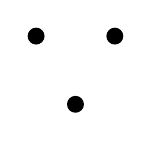
\begin{tikzpicture}[every node/.style = {draw = black, shape = circle, fill, inner sep = 0pt, minimum size = .2cm}]
    	%\node[shape = circle, draw = black, fill] (A) at (-1,0) {};
    	\node (A) at (-.5,0) {};
    	\node (B) at (.5,0) {};
    	\node (C) at (0, -.866) {};
    \end{tikzpicture}
    \vspace{.3cm}
    \caption*{$(1, 0) = \bf{3}$}
    \end{subfigure}
~
	\begin{subfigure}[t]{.3\textwidth}
	\centering
    	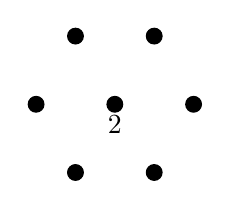
\begin{tikzpicture}[every node/.style = {draw = black, shape = circle, fill, inner sep = 0pt, minimum size = .2cm}]
    	%\node[shape = circle, draw = black, fill] (A) at (-1,0) {};
    	\node (A) at (-1,0) {};
	\node (B) at (-.5, .866) {};
    	\node (C) at (0,0) [label = below:{2}] {};
	\node (D) at (.5, .866) {};
    	\node (E) at (1,0) {};
	\node (F) at (-.5, -.866) {};
	\node (G) at (.5, -.866) {};
    \end{tikzpicture}
    \vspace{.3cm}
    \caption*{$(1, 1) = \bf 8$}
	\end{subfigure}
~
    \begin{subfigure}[t]{.3\textwidth}
    \centering
    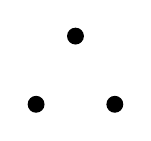
\begin{tikzpicture}[every node/.style = {draw = black, shape = circle, fill, inner sep = 0pt, minimum size = .2cm}]
    	%\node[shape = circle, draw = black, fill] (A) at (-1,0) {};
    	\node (A) at (-.5,0) {};
    	\node (B) at (.5,0) {};
    	\node (C) at (0, .866) {};
    \end{tikzpicture}
    \vspace{.3cm}
    \caption*{$(0, 1) = \bf{\overline{3}}$}
    \end{subfigure}
\end{figure}

\begin{figure}[H]
% \[ \] also works
\centering
    \begin{subfigure}[t]{.3\textwidth}
    \centering
    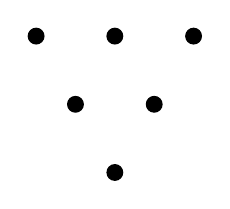
\begin{tikzpicture}[every node/.style = {draw = black, shape = circle, fill, inner sep = 0pt, minimum size = .2cm}]
   	\node (A) at (-.5,0) {};
    	\node (B) at (.5,0) {};
    	\node (C) at (0, .866) {};
	\node (D) at (-1, .866) {};
	\node (E) at (1, .866) {};
	\node (F) at (0, -.866) {};
    \end{tikzpicture}
    \vspace{.3cm}
    \caption*{$(2, 0) = \bf{6}$}
    \end{subfigure}
~
	\begin{subfigure}[t]{.3\textwidth}
	\centering
    	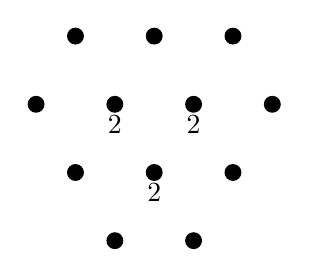
\begin{tikzpicture}[every node/.style = {draw = black, shape = circle, fill, inner sep = 0pt, minimum size = .2cm}]
   	\node (A) at (-.5, .433) [label = below:{2}] {};
    	\node (B) at (.5, .433) [label = below:{2}] {};
    	\node (C) at (0, 1.299) {};
	\node (D) at (-1, 1.299) {};
	\node (E) at (1, 1.299) {};
	\node (F) at (0, -.433) [label = below:{2}] {};
	\node (G) at (-1, -.433) {};
	\node (H) at (1, -.433) {};
   	\node (I) at (-1.5, .433) {};
    	\node (J) at (1.5, .433) {};
   	\node (K) at (-.5, -1.299) {};
    	\node (L) at (.5, -1.299) {};
    \end{tikzpicture}
    \vspace{.3cm}
    \caption*{$(2, 1) = \bf 15$}
	\end{subfigure}
~
    \begin{subfigure}[t]{.3\textwidth}
    \centering
    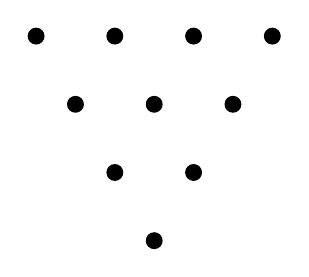
\begin{tikzpicture}[every node/.style = {draw = black, shape = circle, fill, inner sep = 0pt, minimum size = .2cm}]
    	%\node[shape = circle, draw = black, fill] (A) at (-1,0) {};
    	\node (A) at (0, .433) {};
    	\node (B) at (-.5, -.433) {};
    	\node (C) at (.5, -.433) {};
	\node (D) at (-1, .433) {};
	\node (E) at (1, .433) {};
    	\node (F) at (-.5, 1.299) {};
    	\node (G) at (.5, 1.299) {};
    	\node (H) at (-1.5, 1.299) {};
    	\node (I) at (1.5, 1.299) {};
	\node (J) at (0, -1.299) {};
    \end{tikzpicture}
    \vspace{.3cm}
    \caption*{$(3, 0) = \bf{\overline{10}}$}
    \end{subfigure}
\end{figure}

\subsection{Fundamental Representation of SU(N)}

\subsection{General Representations of $SU(N)$}

\subsection{Young Diagrams}


\section{Roots and Weights}
\label{sec:weights}

The general theory of roots and weights we studied in detail for $SU(3)$ will be expanded on in this section.

TODO: relationship between the Cartan subalgebra and Casimir operators? Cartan algebra gives the weights of a 
representation, and for a semisimple algebra the highest weight can be used to label the representation. Casimirs 
also provide a label for the representation though, right?


\newpage
\section{Finite Groups and Characters}

Almost all of the theory we have discussed so far is in application to Lie groups and Lie algebras, which is the basis for how 
we study continuous symmetries in physics. However, it is also important to consider representations of finite groups, as 
these correspond to discrete symmetries. The representation theory of finite groups takes on a slightly different flavor than 
that of Lie groups; it is a bit more combinatorial, and we need to use different machinery than described above with Lie groups 
and algebras. However, the theorems that we are able to prove for finite groups are quite powerful and allow us to 
easily characterize irreps in terms of the order of the group. 

Let $G$ be a finite group, and let $\{D_a : G\rightarrow Aut(V_a)\}_{a\in R(G)}$ be all the irreducible representations of $G$, 
with $R(G)$ indexing the all of these irreps. We will be working towards showing the following results, which will allow us to 
constrain the structure of irreps of $G$ significantly.
 \begin{itemize}
 	\item The set of irreps of $G$ is in bijection with the set of conjugacy classes of $G$. If $Conj(G)$ is the set of conjugacy 
	classes, then:
	\begin{equation}
		|R(G)| = |Conj(G)|
	\end{equation}
	\item For every finite group, we have:
	\begin{equation}
		|G| = \sum_{a\in R(G)} dim(D_a)^2
	\end{equation}
 \end{itemize}

There are a few immediate theorems right off the bat pertaining to finite groups that we will not prove.
\begin{theorem}
	Every representation of a finite group is equivalent to a unitary representation.
\end{theorem}
Since unitary representations are completely reducible, this means that every representation $(D, V)$ of a finite group $G$ is 
completely reducible. So, if we can classify all the irreps of $G$, then we can know exactly every representation of $G$. 

\subsection{Characters}

\subsection{The Regular Representation}

Given a finite group $G$, there is a canonical representation of dimension $N = |G|$, called the \textbf{regular representation} 
of $G$, which we can construct as follows. Label an orthonormal basis of $\mathbb R^N$ by the elements in the group 
$|g\rangle$, so $R^N = span\{|g\rangle\}_{g\in G}$. We define the regular representation $D_R : G\rightarrow 
Aut(\mathbb R^N)$ to act on this basis as follows: 
\begin{equation}
	D_R(g)|h\rangle := |gh\rangle
\end{equation}
i.e. $D_R$ implements the group multiplication law. Note that $D_R$ is not an irrep, and as an explicit example of this 
the subspace spanned by $\sum_{g\in G}|g\rangle$ is a proper invariant subspace of $\mathbb R^N$ (this gives the 
trivial irrep). In fact, every irrep of $G$ can be embedded into the regular representation. 

\subsection{Young Diagrams for Finite Groups}

Young diagrams give a nice way to write down the irreducible representations of permutation groups. 

\section{Examples of Finite Groups}

\subsection{The Symmetric Group}

\subsection{The Octahedral Group}

This is the group of symmetries of the 3 dimensional cube, which consists of all the ways one can rotate, twist, and otherwise 
permute the cube. We will consider the group of proper symmetries of the cube, in which parity is not included. This is 
known as the proper octahedral group and we will denote it by $O_h^+$, as opposed to the full octahedral group, which 
is denoted by $O_h$. The order of $O_h^+$ is 24, and it has 5 conjugacy classes, hence 5 irreps. 

TODO extend to $O_h$. 

\subsection{The Hypercubic Group}

The proper hypercubic group $H(4)^+$ (not including parity) has order 192 and 13 conjugacy classes, hence 13 irreducible 
representations. By adding parity to $H(4)^+$, we get the full hypercubic group $H(4)$. We first discuss the irreps of 
$H(4)^+$, then we will discuss how to extend them to $H(4)$, which is more complicated than the cubic case. 

\end{document}